\chapter{Statistics}\label{chapter:statistics}

\section{Systematic uncertainties and statistical treatment\label{sec:uncertainties}}
\subsection{Detector systematic uncertainties\label{sec:detector_systematics}}
\begingroup
\graphicspath{{results/HESE_Final_Paper/}}
\input{results/HESE_Final_Paper/sections/uncertainties/systematics}
\endgroup

\subsection{Statistical treatment\label{sec:statistics}}
\begingroup
\graphicspath{{results/HESE_Final_Paper/}}
\chapter{Statistics}\label{chapter:statistics}

\section{Systematic uncertainties and statistical treatment\label{sec:uncertainties}}
\subsection{Detector systematic uncertainties\label{sec:detector_systematics}}
\begingroup
\graphicspath{{results/HESE_Final_Paper/}}
\input{results/HESE_Final_Paper/sections/uncertainties/systematics}
\endgroup

\subsection{Statistical treatment\label{sec:statistics}}
\begingroup
\graphicspath{{results/HESE_Final_Paper/}}
\chapter{Statistics}\label{chapter:statistics}

\section{Systematic uncertainties and statistical treatment\label{sec:uncertainties}}
\subsection{Detector systematic uncertainties\label{sec:detector_systematics}}
\begingroup
\graphicspath{{results/HESE_Final_Paper/}}
\input{results/HESE_Final_Paper/sections/uncertainties/systematics}
\endgroup

\subsection{Statistical treatment\label{sec:statistics}}
\begingroup
\graphicspath{{results/HESE_Final_Paper/}}
\chapter{Statistics}\label{chapter:statistics}

\section{Systematic uncertainties and statistical treatment\label{sec:uncertainties}}
\subsection{Detector systematic uncertainties\label{sec:detector_systematics}}
\begingroup
\graphicspath{{results/HESE_Final_Paper/}}
\input{results/HESE_Final_Paper/sections/uncertainties/systematics}
\endgroup

\subsection{Statistical treatment\label{sec:statistics}}
\begingroup
\graphicspath{{results/HESE_Final_Paper/}}
\input{results/HESE_Final_Paper/sections/uncertainties/statistics}
\endgroup

\section{Dealing with limited simulation samples\label{sec:limited_simulation}}
The contents of this section is reproduced here with minor modifications from a collaborative work with Carlos A. Argüelles, and Tianlu Yuan~\cite{Arguelles:2019izp}.

\begingroup
\graphicspath{{results/mcllh_paper/}}
\input{results/mcllh_paper/sections/introduction}
\endgroup

\subsection{The Poisson likelihood and previous work\label{sec:mc_intro}}
\begingroup
\graphicspath{{results/mcllh_paper/}}
\input{results/mcllh_paper/sections/previous_work/poisson}
\endgroup

\subsubsection{The Barlow-Beeston likelihood}
\begingroup
\graphicspath{{results/mcllh_paper/}}
\input{results/mcllh_paper/sections/previous_work/bb}
\endgroup

\subsubsection{Uncertainties in the large-sample limit}
\begingroup
\graphicspath{{results/mcllh_paper/}}
\input{results/mcllh_paper/sections/previous_work/chi2}
\endgroup

\subsection{Generalization of the Poisson likelihood\label{sec:generalization_poisson}}
\begingroup
\graphicspath{{results/mcllh_paper/}}
\input{results/mcllh_paper/sections/generalized_poisson/generalized_poisson}
\endgroup

\subsubsection{Derivation of $\like (\lambda|\vecw(\vectheta))$ for identical weights\label{sec:constructing}}
\begingroup
\graphicspath{{results/mcllh_paper/}}
\input{results/mcllh_paper/sections/generalized_poisson/identical_weights}
\endgroup

\subsubsection{Extension to arbitrary weights\label{sec:extending}}
\begingroup
\graphicspath{{results/mcllh_paper/}}
\input{results/mcllh_paper/sections/generalized_poisson/arbitrary_weights}
\endgroup

\subsubsection{The effective likelihood\label{sec:effective}}
\begingroup
\graphicspath{{results/mcllh_paper/}}
\input{results/mcllh_paper/sections/generalized_poisson/effective_likelihood}
\endgroup

\subsubsection{A family of likelihoods\label{sec:priors}}
\begingroup
\graphicspath{{results/mcllh_paper/}}
\input{results/mcllh_paper/sections/generalized_poisson/family}
\endgroup

\subsubsection{Convergence of the effective likelihood\label{sec:llhconvergence}}
\begingroup
\graphicspath{{results/mcllh_paper/}}
\input{results/mcllh_paper/sections/generalized_poisson/convergence}
\endgroup

\subsubsection{Behavior of the effective likelihood\label{sec:llhbehavior}}
\begingroup
\graphicspath{{results/mcllh_paper/}}
\input{results/mcllh_paper/sections/generalized_poisson/behavior}
\endgroup

\subsection{Example and performance\label{sec:example}}
\begingroup
\graphicspath{{results/mcllh_paper/}}
\input{results/mcllh_paper/sections/example/example}
\endgroup

\subsubsection{Point estimation\label{sec:pointestimation}}
\begingroup
\graphicspath{{results/mcllh_paper/}}
\input{results/mcllh_paper/sections/example/point_estimation}
\endgroup

\subsubsection{Coverage\label{sec:coverage}}
\begingroup
\graphicspath{{results/mcllh_paper/}}
\input{results/mcllh_paper/sections/example/coverage}
\endgroup

\subsubsection{Posterior distributions\label{sec:posterior}}
\begingroup
\graphicspath{{results/mcllh_paper/}}
\input{results/mcllh_paper/sections/example/posterior}
\endgroup

\subsubsection{Performance\label{sec:performance}}
\begingroup
\graphicspath{{results/mcllh_paper/}}
\input{results/mcllh_paper/sections/example/performance}
\endgroup

\subsection{Conclusion\label{sec:llhconclusion}}
\begingroup
\graphicspath{{results/mcllh_paper/}}
\input{results/mcllh_paper/sections/conclusion}
\endgroup

\subsection{Summary of likelihood formulas\label{sec:llhtable}}
\begingroup
\graphicspath{{results/mcllh_paper/}}
\input{results/mcllh_paper/appendices/formulas}
\endgroup
\FloatBarrier
\section{Frequentist confidence intervals with nuisance parameters and limited simulation}\label{sec:low_stats_confidence_intervals}

Frequentist and Bayesian techniques deal with different two different kinds of probability.
In frequentist statistics, the relevant probability is the frequency of the outcome of a repeatable experiment.
Under this framework the important concepts are parameter estimation, confidence intervals, and statistical tests.
In Bayesian statistics, the relevant probabilities come from the application of Bayes theorem which means we can define the probability density of parameters.
This definition of the parameter p.d.f. is applicable to the same problems parameter estimation, interval construction, and statistical tests but comes at the cost of defining ``prior belief'' about parameters.

In this section we will ignore the problem of statistical tests, instead focusing on the common features that underpin parameter estimation and interval construction.
Generally in parameter estimation and interval construction there are two sets of parameters, parameters of interest $\vec\theta$ and nuisance parameters $\vec\eta$.
Fundamentally there is no distinction between these two kinds of parameters.
The difference is only in which parameters we want to infer information about.

For both parameter estimation and interval construction the likelihood function is central.
The likelihood function reflects the plausibility of model parameters given observed data and is defined as $\like(\vec\theta, \vec\eta|\textrm{data}) = p(\textrm{data}|\vec\theta, \vec\eta)$.
Where $p(\textrm{data}|\vec\theta, \vec\eta)$ is the probability of the data given the model parameters.
A useful technique to eliminate nuisance parameters is the profile likelihood technique.
Dropping the explicit notational dependence on data, the profile likelihood function is defined as
\begin{linenomath*}
	\begin{equation}
	\tilde{\like}^\texttt{profile}(\vec\theta) = \max_{\vec\eta} \like(\vec\theta,\vec\eta),
	\label{eq:likelihood_profile}
	\end{equation}
\end{linenomath*}
where often the negative log of the function is maximized in place of the function for computational reasons.
The profile likelihood is then only a function of the parameters of interest.
Parameter estimation can be performed by maximizing the profile likelihood to obtain the ``best-fit'' parameters
\begin{linenomath*}
	\begin{equation}
	\hat{\vec\theta} = \argmax_{\vec\theta} \tilde{\like}^\texttt{profile}(\vec\theta).
	\label{eq:best_fit}
	\end{equation}
\end{linenomath*}
This best-fit point in the parameter space is a derived property of the likelihood function.
However, the same procedure can be performed with other functions to the same effect.
In general a minimization procedure is used, and we refer to these functions as ``test-statistics'' (TS).
A particularly useful TS is derived directly from the profile likelihood technique,
\begin{linenomath*}
	\begin{equation}
	\TS(\vec\theta) = -2\log{\left(\frac{\tilde{\like}^\texttt{profile}(\vec\theta)}{\tilde{\like}^\texttt{profile}(\hat{\vec\theta})}\right)}.
	\end{equation}
\end{linenomath*}
Using this TS to perform parameter estimation through minimization is mathematically equivalent to maximizing the likelihood, however, this form will prove to be uniquely useful for interval construction.

Since frequentist statistics deals with the frequency of outcomes from repeated experiments we can use the TS that results from repeated experiments to construct probabilities.
Consider for a moment a single point in the parameter space $\vec\theta_0$.
At this point in the parameter space there is a distribution of data that can be observed, and therefore a distribution of TS functions.
Instead of considering the distribution of TS functions originating from this point, we can simplify the picture by looking at the TS function only evaluated at this point $\TS(\vec\theta_0)$.
This gives us a distribution of TS values for this point in the parameter space that may look like~\reffig{fig:TS_dist}.
\begin{figure}
	\centering
	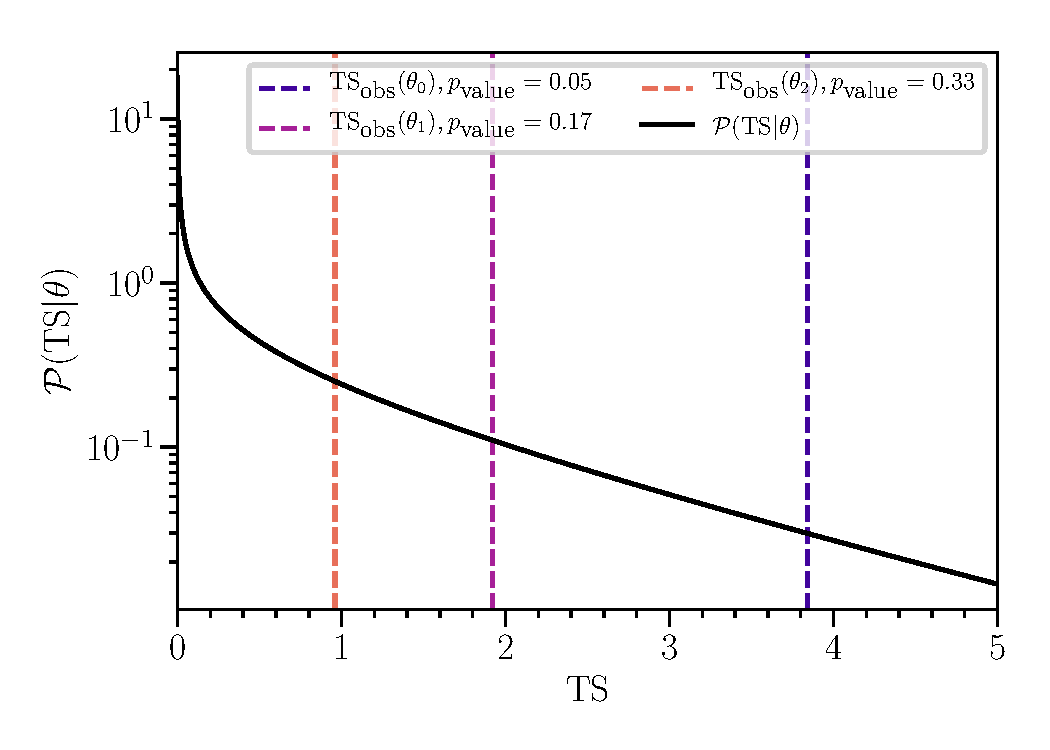
\includegraphics[width=0.8\linewidth]{figures/TS_dist}
	\caption{\textbf{\textit{Test statistic distribution.}} An example of a test statistic distribution.
	Such distributions tend to have the bulk of their mass close to the lower boundary with a long tail.
	Lower values indicate better statistical compatibility with the data.
	}
	\label{fig:TS_dist}
\end{figure}
It is important to note that for the profile likelihood TS and similar statistics a smaller TS value indicates better compatibility with the data.
For this reason many statistical tests are constructed using a single tail significance, by comparing the TS from a single experiment to a background TS distribution and reporting a p-value that is the fraction of the TS distribution greater than the observed TS.

This procedure can be extended to construct intervals by considering the TS distributions of every point in parameter space and comparing to the observed TS function.
Consider the one-dimensional case where there is a TS distribution for each value of the parameter, illustrated in~\reffig{fig:TS_dists_1d}
\begin{figure}
	\centering
	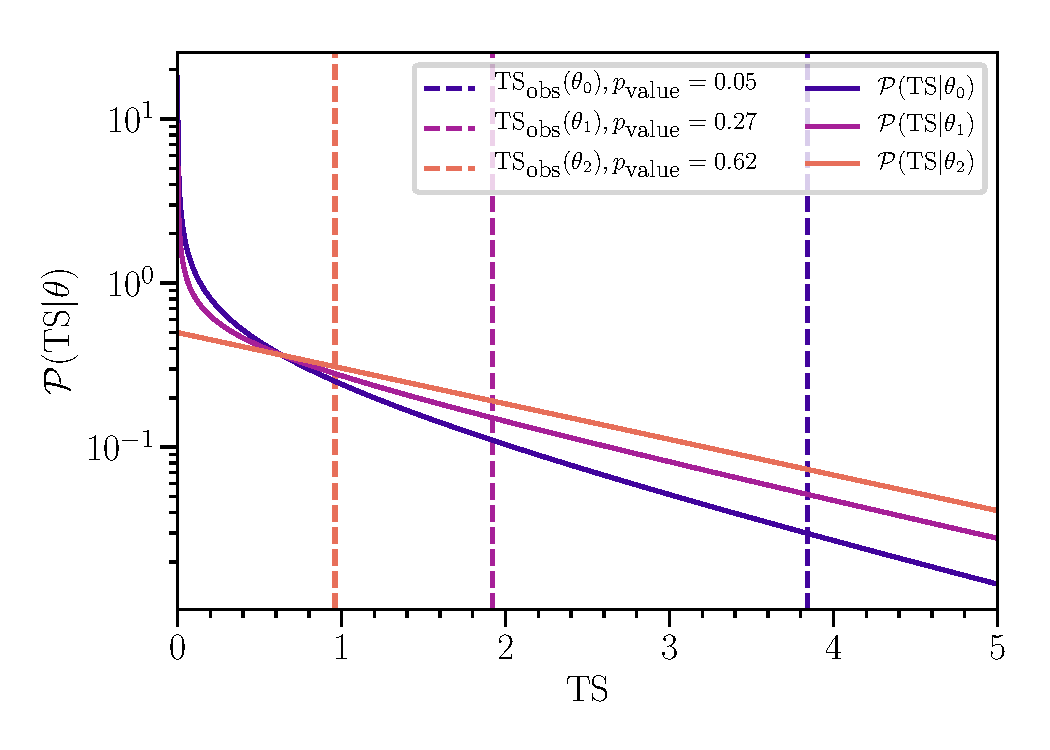
\includegraphics[width=0.8\linewidth]{figures/TS_dists_1d}
	\caption{\textbf{\textit{One-dimensional test-statistic distribution comparison.}} An example of the test statistic distributions as a function of a single parameter.
	}
	\label{fig:TS_dists_1d}
\end{figure}
We can construct an interval that will contain the true value of the parameter a fraction of the time $\alpha$ for repeated experiments.
This interval is the collection of points in the one-dimensional parameter space where the TS at that point is greater than the $\alpha$ quantile of the corresponding TS distribution.
If the TS distribution is the same for all points in parameter space, the interval construction can procedurally be thought of as drawing a horizontal line at the appropriate threshold and only including points that lie below the line.
Varying TS distributions modify this procedure to the comparison of two curves.
This procedure is not limited to one-dimension but can be extended to an arbitrary number of parameters of interest to construct n-dimensional regions with the same properties.

There is however an important caveat to this construction that appears when we consider nuisance parameters.
In order for the intervals to have the desired properties, the observed TS must be greater than the threshold for all possible values of the nuisance parameters.
This ultimatum presents several challenges.
Nuisance parameters can often have a broad or even unbounded range of allowed values, meaning if the effect of nuisance parameters does not taper off at the extrema then almost all intervals are guaranteed to be empty.
From a practical standpoint, computing the TS distributions for many points in parameter space is often done via Monte-Carlo and is computationally expensive.
Adding additional dimensions to the parameter space for which we must compute TS distributions exponentially increases the computation time.

To combat these issues we can limit our interval construction to be valid for values of the nuisance parameters that are ``reasonable''.
There are several methods for doing this, but we can split them into two categories: pure frequentist, and frequentist-Bayesian hybrid.
In the pure frequentist approaches we can either choose a single value of the nuisance parameters, or work with a limited range of the nuisance parameter values.
For the single value approach either nominal values are chosen before looking at the data, or estimators of the nuisance parameters are used to choose their values.
This approach benefits from simplicity, but fails if the test-statistic distributions vary rapidly with changes to the nuisance parameters for values that we might consider ``reasonable''.
A more expensive but robust approach is to explore the behavior of TS distributions for a limited range of the nuisance parameter values, which can be chosen {\it a priori} or from data-based bounds on the nuisance parameters.
If we are willing to consider a hybrid approach, then some more pragmatic options are available.

Although Bayesian methods could be used to choose a single point in parameter space from which to generate the TS distributions, the more interesting application is one that uses a distribution in parameter space.
In Bayesian statistics we can directly assign a probability density to the points in parameter space, either based on our prior information, or directly informed by the posterior distribution, from this extended perspective the probability of certain nuisance parameter values is of interest when considering the frequency of TS values for different parameters of interest.
The prior case is simple in that we sample the from the nuisance parameter priors when generating the TS distribution which allows us to account for variability introduced by the nuisance parameters without relying on hard cutoffs or biasing our inferences with parameter values that are unrealistic.
This prior based technique is well motivated if the priors are derived from external observations, however in the case where nuisance parameters have broad or ``uninformative'' priors this motivation and benefit may break down.
In some cases we expect nuisance parameters to be heavily constrained by the same data sample used to investigate the parameters of interest, so a different approach is merited.
The alternative is to use the posterior distribution to construct our nuisance parameter p.d.f.
Ideally a posterior distribution would be computed for each point in the parameters of interest space by fixing those parameters of interest.
In this way the nuisance parameter posterior used for sampling depends on the point in parameter space we are examining.

With the possible solutions available, we can now look at the problem of limited simulation size when generating test statistic distributions.
As explored in~\refsec{sec:limited_simulation} for binned Poisson likelihood problems, the real expectation in data or simulation for the number of events in a bin is not a known quantity.
Because the real expectations are not known, it is impossible to exactly model the distribution of TS that are expected for a particular point in the parameter space.
However, as~\refsec{sec:limited_simulation} also explored, limited simulation can be modeled with nuisance parameters so the techniques discussed above can be applied directly to the problem.
The ``single point in parameter space'' approach fails to address the additional uncertainty present in this case.
Allowing for unbounded variation of the bin expectations fails as it is guaranteed to produce empty intervals.
Bounding of the bin expectations within a reasonable range provides manageable intervals, but the dimensionality of the problem makes this computationally unfeasible beyond a handful of bins.
Unfortunately this excludes all the ``classic'' frequentist solutions to this problem.
The hybrid Bayesian-frequentist methods in this case provide a tractable solution that accounts for the additional uncertainty.
We can make use of the treatment described in~\refsec{sec:effective}, where the bin expectation is derived to be gamma distributed, and the expected number of data events modeled to be Poisson distributed once this expectation is known.
Practically this can be achieved by sampling data events from $\mcl$, or through a two step process where the expectation is sampled from a gamma distribution $\gprob(\lambda;\agpar, \bgpar)$ where $\agpar = \frac{\mu^2}{\sigma^2}+1~\textmd{and}~\bgpar=\frac{\mu}{\sigma^2}$, and the data events are sampled from a Poisson distribution $\frac{\lambda^{k}e^{-\lambda}}{k!}$.
It is important to note that this procedure only applies to variations in the data and should not be used to vary simulation expectations.
This is because the TS distribution is intended to model variations in the data, whereas the simulation used for analysis is fixed.
Combined with a similar hybrid treatment for other nuisance parameters, this provides a more complete accounting of the uncertainties given the available modeling.
\endgroup

\section{Dealing with limited simulation samples\label{sec:limited_simulation}}
The contents of this section is reproduced here with minor modifications from a collaborative work with Carlos A. Argüelles, and Tianlu Yuan~\cite{Arguelles:2019izp}.

\begingroup
\graphicspath{{results/mcllh_paper/}}
\chapter{Introduction}


\endgroup

\subsection{The Poisson likelihood and previous work\label{sec:mc_intro}}
\begingroup
\graphicspath{{results/mcllh_paper/}}
\input{results/mcllh_paper/sections/previous_work/poisson}
\endgroup

\subsubsection{The Barlow-Beeston likelihood}
\begingroup
\graphicspath{{results/mcllh_paper/}}
\input{results/mcllh_paper/sections/previous_work/bb}
\endgroup

\subsubsection{Uncertainties in the large-sample limit}
\begingroup
\graphicspath{{results/mcllh_paper/}}
\input{results/mcllh_paper/sections/previous_work/chi2}
\endgroup

\subsection{Generalization of the Poisson likelihood\label{sec:generalization_poisson}}
\begingroup
\graphicspath{{results/mcllh_paper/}}
\input{results/mcllh_paper/sections/generalized_poisson/generalized_poisson}
\endgroup

\subsubsection{Derivation of $\like (\lambda|\vecw(\vectheta))$ for identical weights\label{sec:constructing}}
\begingroup
\graphicspath{{results/mcllh_paper/}}
\input{results/mcllh_paper/sections/generalized_poisson/identical_weights}
\endgroup

\subsubsection{Extension to arbitrary weights\label{sec:extending}}
\begingroup
\graphicspath{{results/mcllh_paper/}}
\input{results/mcllh_paper/sections/generalized_poisson/arbitrary_weights}
\endgroup

\subsubsection{The effective likelihood\label{sec:effective}}
\begingroup
\graphicspath{{results/mcllh_paper/}}
\input{results/mcllh_paper/sections/generalized_poisson/effective_likelihood}
\endgroup

\subsubsection{A family of likelihoods\label{sec:priors}}
\begingroup
\graphicspath{{results/mcllh_paper/}}
\input{results/mcllh_paper/sections/generalized_poisson/family}
\endgroup

\subsubsection{Convergence of the effective likelihood\label{sec:llhconvergence}}
\begingroup
\graphicspath{{results/mcllh_paper/}}
\input{results/mcllh_paper/sections/generalized_poisson/convergence}
\endgroup

\subsubsection{Behavior of the effective likelihood\label{sec:llhbehavior}}
\begingroup
\graphicspath{{results/mcllh_paper/}}
\input{results/mcllh_paper/sections/generalized_poisson/behavior}
\endgroup

\subsection{Example and performance\label{sec:example}}
\begingroup
\graphicspath{{results/mcllh_paper/}}
\input{results/mcllh_paper/sections/example/example}
\endgroup

\subsubsection{Point estimation\label{sec:pointestimation}}
\begingroup
\graphicspath{{results/mcllh_paper/}}
\input{results/mcllh_paper/sections/example/point_estimation}
\endgroup

\subsubsection{Coverage\label{sec:coverage}}
\begingroup
\graphicspath{{results/mcllh_paper/}}
\input{results/mcllh_paper/sections/example/coverage}
\endgroup

\subsubsection{Posterior distributions\label{sec:posterior}}
\begingroup
\graphicspath{{results/mcllh_paper/}}
\input{results/mcllh_paper/sections/example/posterior}
\endgroup

\subsubsection{Performance\label{sec:performance}}
\begingroup
\graphicspath{{results/mcllh_paper/}}
\input{results/mcllh_paper/sections/example/performance}
\endgroup

\subsection{Conclusion\label{sec:llhconclusion}}
\begingroup
\graphicspath{{results/mcllh_paper/}}
\input{results/mcllh_paper/sections/conclusion}
\endgroup

\subsection{Summary of likelihood formulas\label{sec:llhtable}}
\begingroup
\graphicspath{{results/mcllh_paper/}}
\input{results/mcllh_paper/appendices/formulas}
\endgroup
\FloatBarrier
\section{Frequentist confidence intervals with nuisance parameters and limited simulation}\label{sec:low_stats_confidence_intervals}

Frequentist and Bayesian techniques deal with different two different kinds of probability.
In frequentist statistics, the relevant probability is the frequency of the outcome of a repeatable experiment.
Under this framework the important concepts are parameter estimation, confidence intervals, and statistical tests.
In Bayesian statistics, the relevant probabilities come from the application of Bayes theorem which means we can define the probability density of parameters.
This definition of the parameter p.d.f. is applicable to the same problems parameter estimation, interval construction, and statistical tests but comes at the cost of defining ``prior belief'' about parameters.

In this section we will ignore the problem of statistical tests, instead focusing on the common features that underpin parameter estimation and interval construction.
Generally in parameter estimation and interval construction there are two sets of parameters, parameters of interest $\vec\theta$ and nuisance parameters $\vec\eta$.
Fundamentally there is no distinction between these two kinds of parameters.
The difference is only in which parameters we want to infer information about.

For both parameter estimation and interval construction the likelihood function is central.
The likelihood function reflects the plausibility of model parameters given observed data and is defined as $\like(\vec\theta, \vec\eta|\textrm{data}) = p(\textrm{data}|\vec\theta, \vec\eta)$.
Where $p(\textrm{data}|\vec\theta, \vec\eta)$ is the probability of the data given the model parameters.
A useful technique to eliminate nuisance parameters is the profile likelihood technique.
Dropping the explicit notational dependence on data, the profile likelihood function is defined as
\begin{linenomath*}
	\begin{equation}
	\tilde{\like}^\texttt{profile}(\vec\theta) = \max_{\vec\eta} \like(\vec\theta,\vec\eta),
	\label{eq:likelihood_profile}
	\end{equation}
\end{linenomath*}
where often the negative log of the function is maximized in place of the function for computational reasons.
The profile likelihood is then only a function of the parameters of interest.
Parameter estimation can be performed by maximizing the profile likelihood to obtain the ``best-fit'' parameters
\begin{linenomath*}
	\begin{equation}
	\hat{\vec\theta} = \argmax_{\vec\theta} \tilde{\like}^\texttt{profile}(\vec\theta).
	\label{eq:best_fit}
	\end{equation}
\end{linenomath*}
This best-fit point in the parameter space is a derived property of the likelihood function.
However, the same procedure can be performed with other functions to the same effect.
In general a minimization procedure is used, and we refer to these functions as ``test-statistics'' (TS).
A particularly useful TS is derived directly from the profile likelihood technique,
\begin{linenomath*}
	\begin{equation}
	\TS(\vec\theta) = -2\log{\left(\frac{\tilde{\like}^\texttt{profile}(\vec\theta)}{\tilde{\like}^\texttt{profile}(\hat{\vec\theta})}\right)}.
	\end{equation}
\end{linenomath*}
Using this TS to perform parameter estimation through minimization is mathematically equivalent to maximizing the likelihood, however, this form will prove to be uniquely useful for interval construction.

Since frequentist statistics deals with the frequency of outcomes from repeated experiments we can use the TS that results from repeated experiments to construct probabilities.
Consider for a moment a single point in the parameter space $\vec\theta_0$.
At this point in the parameter space there is a distribution of data that can be observed, and therefore a distribution of TS functions.
Instead of considering the distribution of TS functions originating from this point, we can simplify the picture by looking at the TS function only evaluated at this point $\TS(\vec\theta_0)$.
This gives us a distribution of TS values for this point in the parameter space that may look like~\reffig{fig:TS_dist}.
\begin{figure}
	\centering
	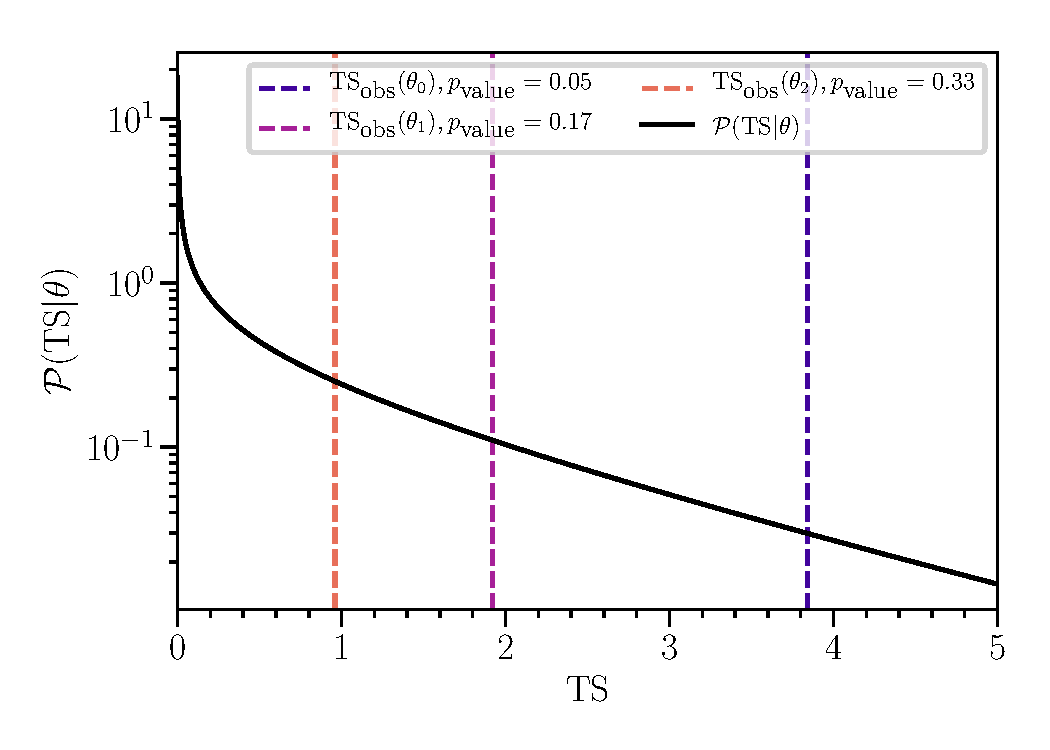
\includegraphics[width=0.8\linewidth]{figures/TS_dist}
	\caption{\textbf{\textit{Test statistic distribution.}} An example of a test statistic distribution.
	Such distributions tend to have the bulk of their mass close to the lower boundary with a long tail.
	Lower values indicate better statistical compatibility with the data.
	}
	\label{fig:TS_dist}
\end{figure}
It is important to note that for the profile likelihood TS and similar statistics a smaller TS value indicates better compatibility with the data.
For this reason many statistical tests are constructed using a single tail significance, by comparing the TS from a single experiment to a background TS distribution and reporting a p-value that is the fraction of the TS distribution greater than the observed TS.

This procedure can be extended to construct intervals by considering the TS distributions of every point in parameter space and comparing to the observed TS function.
Consider the one-dimensional case where there is a TS distribution for each value of the parameter, illustrated in~\reffig{fig:TS_dists_1d}
\begin{figure}
	\centering
	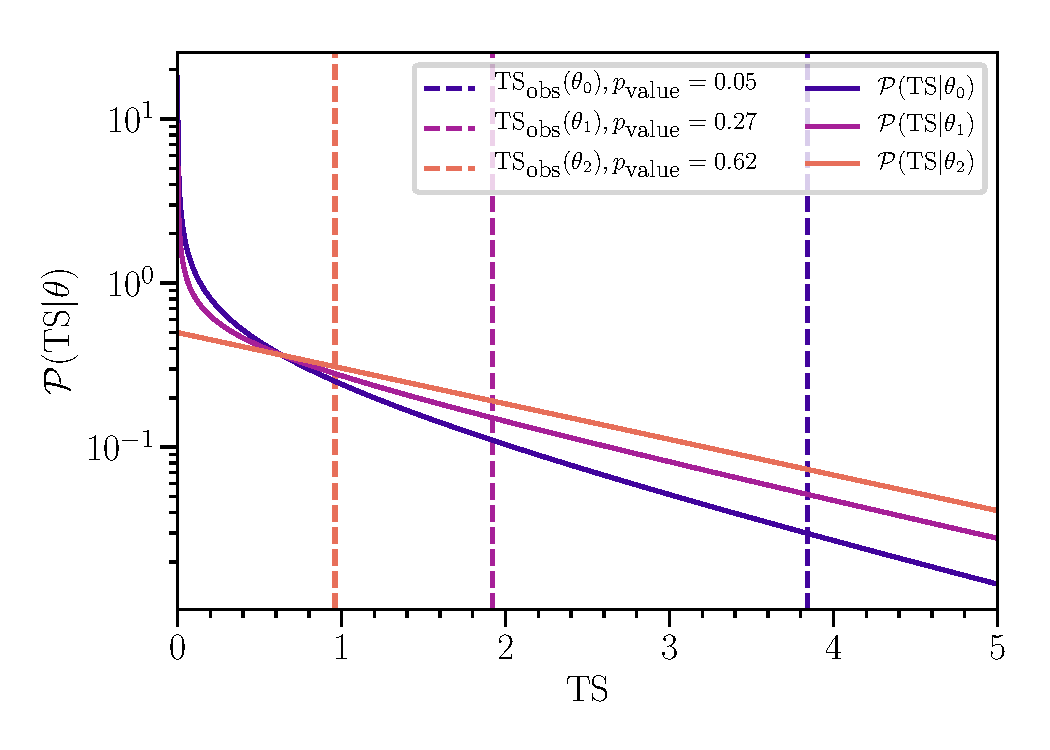
\includegraphics[width=0.8\linewidth]{figures/TS_dists_1d}
	\caption{\textbf{\textit{One-dimensional test-statistic distribution comparison.}} An example of the test statistic distributions as a function of a single parameter.
	}
	\label{fig:TS_dists_1d}
\end{figure}
We can construct an interval that will contain the true value of the parameter a fraction of the time $\alpha$ for repeated experiments.
This interval is the collection of points in the one-dimensional parameter space where the TS at that point is greater than the $\alpha$ quantile of the corresponding TS distribution.
If the TS distribution is the same for all points in parameter space, the interval construction can procedurally be thought of as drawing a horizontal line at the appropriate threshold and only including points that lie below the line.
Varying TS distributions modify this procedure to the comparison of two curves.
This procedure is not limited to one-dimension but can be extended to an arbitrary number of parameters of interest to construct n-dimensional regions with the same properties.

There is however an important caveat to this construction that appears when we consider nuisance parameters.
In order for the intervals to have the desired properties, the observed TS must be greater than the threshold for all possible values of the nuisance parameters.
This ultimatum presents several challenges.
Nuisance parameters can often have a broad or even unbounded range of allowed values, meaning if the effect of nuisance parameters does not taper off at the extrema then almost all intervals are guaranteed to be empty.
From a practical standpoint, computing the TS distributions for many points in parameter space is often done via Monte-Carlo and is computationally expensive.
Adding additional dimensions to the parameter space for which we must compute TS distributions exponentially increases the computation time.

To combat these issues we can limit our interval construction to be valid for values of the nuisance parameters that are ``reasonable''.
There are several methods for doing this, but we can split them into two categories: pure frequentist, and frequentist-Bayesian hybrid.
In the pure frequentist approaches we can either choose a single value of the nuisance parameters, or work with a limited range of the nuisance parameter values.
For the single value approach either nominal values are chosen before looking at the data, or estimators of the nuisance parameters are used to choose their values.
This approach benefits from simplicity, but fails if the test-statistic distributions vary rapidly with changes to the nuisance parameters for values that we might consider ``reasonable''.
A more expensive but robust approach is to explore the behavior of TS distributions for a limited range of the nuisance parameter values, which can be chosen {\it a priori} or from data-based bounds on the nuisance parameters.
If we are willing to consider a hybrid approach, then some more pragmatic options are available.

Although Bayesian methods could be used to choose a single point in parameter space from which to generate the TS distributions, the more interesting application is one that uses a distribution in parameter space.
In Bayesian statistics we can directly assign a probability density to the points in parameter space, either based on our prior information, or directly informed by the posterior distribution, from this extended perspective the probability of certain nuisance parameter values is of interest when considering the frequency of TS values for different parameters of interest.
The prior case is simple in that we sample the from the nuisance parameter priors when generating the TS distribution which allows us to account for variability introduced by the nuisance parameters without relying on hard cutoffs or biasing our inferences with parameter values that are unrealistic.
This prior based technique is well motivated if the priors are derived from external observations, however in the case where nuisance parameters have broad or ``uninformative'' priors this motivation and benefit may break down.
In some cases we expect nuisance parameters to be heavily constrained by the same data sample used to investigate the parameters of interest, so a different approach is merited.
The alternative is to use the posterior distribution to construct our nuisance parameter p.d.f.
Ideally a posterior distribution would be computed for each point in the parameters of interest space by fixing those parameters of interest.
In this way the nuisance parameter posterior used for sampling depends on the point in parameter space we are examining.

With the possible solutions available, we can now look at the problem of limited simulation size when generating test statistic distributions.
As explored in~\refsec{sec:limited_simulation} for binned Poisson likelihood problems, the real expectation in data or simulation for the number of events in a bin is not a known quantity.
Because the real expectations are not known, it is impossible to exactly model the distribution of TS that are expected for a particular point in the parameter space.
However, as~\refsec{sec:limited_simulation} also explored, limited simulation can be modeled with nuisance parameters so the techniques discussed above can be applied directly to the problem.
The ``single point in parameter space'' approach fails to address the additional uncertainty present in this case.
Allowing for unbounded variation of the bin expectations fails as it is guaranteed to produce empty intervals.
Bounding of the bin expectations within a reasonable range provides manageable intervals, but the dimensionality of the problem makes this computationally unfeasible beyond a handful of bins.
Unfortunately this excludes all the ``classic'' frequentist solutions to this problem.
The hybrid Bayesian-frequentist methods in this case provide a tractable solution that accounts for the additional uncertainty.
We can make use of the treatment described in~\refsec{sec:effective}, where the bin expectation is derived to be gamma distributed, and the expected number of data events modeled to be Poisson distributed once this expectation is known.
Practically this can be achieved by sampling data events from $\mcl$, or through a two step process where the expectation is sampled from a gamma distribution $\gprob(\lambda;\agpar, \bgpar)$ where $\agpar = \frac{\mu^2}{\sigma^2}+1~\textmd{and}~\bgpar=\frac{\mu}{\sigma^2}$, and the data events are sampled from a Poisson distribution $\frac{\lambda^{k}e^{-\lambda}}{k!}$.
It is important to note that this procedure only applies to variations in the data and should not be used to vary simulation expectations.
This is because the TS distribution is intended to model variations in the data, whereas the simulation used for analysis is fixed.
Combined with a similar hybrid treatment for other nuisance parameters, this provides a more complete accounting of the uncertainties given the available modeling.
\endgroup

\section{Dealing with limited simulation samples\label{sec:limited_simulation}}
The contents of this section is reproduced here with minor modifications from a collaborative work with Carlos A. Argüelles, and Tianlu Yuan~\cite{Arguelles:2019izp}.

\begingroup
\graphicspath{{results/mcllh_paper/}}
\chapter{Introduction}


\endgroup

\subsection{The Poisson likelihood and previous work\label{sec:mc_intro}}
\begingroup
\graphicspath{{results/mcllh_paper/}}
\input{results/mcllh_paper/sections/previous_work/poisson}
\endgroup

\subsubsection{The Barlow-Beeston likelihood}
\begingroup
\graphicspath{{results/mcllh_paper/}}
\input{results/mcllh_paper/sections/previous_work/bb}
\endgroup

\subsubsection{Uncertainties in the large-sample limit}
\begingroup
\graphicspath{{results/mcllh_paper/}}
\input{results/mcllh_paper/sections/previous_work/chi2}
\endgroup

\subsection{Generalization of the Poisson likelihood\label{sec:generalization_poisson}}
\begingroup
\graphicspath{{results/mcllh_paper/}}
\input{results/mcllh_paper/sections/generalized_poisson/generalized_poisson}
\endgroup

\subsubsection{Derivation of $\like (\lambda|\vecw(\vectheta))$ for identical weights\label{sec:constructing}}
\begingroup
\graphicspath{{results/mcllh_paper/}}
\input{results/mcllh_paper/sections/generalized_poisson/identical_weights}
\endgroup

\subsubsection{Extension to arbitrary weights\label{sec:extending}}
\begingroup
\graphicspath{{results/mcllh_paper/}}
\input{results/mcllh_paper/sections/generalized_poisson/arbitrary_weights}
\endgroup

\subsubsection{The effective likelihood\label{sec:effective}}
\begingroup
\graphicspath{{results/mcllh_paper/}}
\input{results/mcllh_paper/sections/generalized_poisson/effective_likelihood}
\endgroup

\subsubsection{A family of likelihoods\label{sec:priors}}
\begingroup
\graphicspath{{results/mcllh_paper/}}
\input{results/mcllh_paper/sections/generalized_poisson/family}
\endgroup

\subsubsection{Convergence of the effective likelihood\label{sec:llhconvergence}}
\begingroup
\graphicspath{{results/mcllh_paper/}}
\input{results/mcllh_paper/sections/generalized_poisson/convergence}
\endgroup

\subsubsection{Behavior of the effective likelihood\label{sec:llhbehavior}}
\begingroup
\graphicspath{{results/mcllh_paper/}}
\input{results/mcllh_paper/sections/generalized_poisson/behavior}
\endgroup

\subsection{Example and performance\label{sec:example}}
\begingroup
\graphicspath{{results/mcllh_paper/}}
\input{results/mcllh_paper/sections/example/example}
\endgroup

\subsubsection{Point estimation\label{sec:pointestimation}}
\begingroup
\graphicspath{{results/mcllh_paper/}}
\input{results/mcllh_paper/sections/example/point_estimation}
\endgroup

\subsubsection{Coverage\label{sec:coverage}}
\begingroup
\graphicspath{{results/mcllh_paper/}}
\input{results/mcllh_paper/sections/example/coverage}
\endgroup

\subsubsection{Posterior distributions\label{sec:posterior}}
\begingroup
\graphicspath{{results/mcllh_paper/}}
\input{results/mcllh_paper/sections/example/posterior}
\endgroup

\subsubsection{Performance\label{sec:performance}}
\begingroup
\graphicspath{{results/mcllh_paper/}}
\input{results/mcllh_paper/sections/example/performance}
\endgroup

\subsection{Conclusion\label{sec:llhconclusion}}
\begingroup
\graphicspath{{results/mcllh_paper/}}
\input{results/mcllh_paper/sections/conclusion}
\endgroup

\subsection{Summary of likelihood formulas\label{sec:llhtable}}
\begingroup
\graphicspath{{results/mcllh_paper/}}
\input{results/mcllh_paper/appendices/formulas}
\endgroup
\FloatBarrier
\section{Frequentist confidence intervals with nuisance parameters and limited simulation}\label{sec:low_stats_confidence_intervals}

Frequentist and Bayesian techniques deal with different two different kinds of probability.
In frequentist statistics, the relevant probability is the frequency of the outcome of a repeatable experiment.
Under this framework the important concepts are parameter estimation, confidence intervals, and statistical tests.
In Bayesian statistics, the relevant probabilities come from the application of Bayes theorem which means we can define the probability density of parameters.
This definition of the parameter p.d.f. is applicable to the same problems parameter estimation, interval construction, and statistical tests but comes at the cost of defining ``prior belief'' about parameters.

In this section we will ignore the problem of statistical tests, instead focusing on the common features that underpin parameter estimation and interval construction.
Generally in parameter estimation and interval construction there are two sets of parameters, parameters of interest $\vec\theta$ and nuisance parameters $\vec\eta$.
Fundamentally there is no distinction between these two kinds of parameters.
The difference is only in which parameters we want to infer information about.

For both parameter estimation and interval construction the likelihood function is central.
The likelihood function reflects the plausibility of model parameters given observed data and is defined as $\like(\vec\theta, \vec\eta|\textrm{data}) = p(\textrm{data}|\vec\theta, \vec\eta)$.
Where $p(\textrm{data}|\vec\theta, \vec\eta)$ is the probability of the data given the model parameters.
A useful technique to eliminate nuisance parameters is the profile likelihood technique.
Dropping the explicit notational dependence on data, the profile likelihood function is defined as
\begin{linenomath*}
	\begin{equation}
	\tilde{\like}^\texttt{profile}(\vec\theta) = \max_{\vec\eta} \like(\vec\theta,\vec\eta),
	\label{eq:likelihood_profile}
	\end{equation}
\end{linenomath*}
where often the negative log of the function is maximized in place of the function for computational reasons.
The profile likelihood is then only a function of the parameters of interest.
Parameter estimation can be performed by maximizing the profile likelihood to obtain the ``best-fit'' parameters
\begin{linenomath*}
	\begin{equation}
	\hat{\vec\theta} = \argmax_{\vec\theta} \tilde{\like}^\texttt{profile}(\vec\theta).
	\label{eq:best_fit}
	\end{equation}
\end{linenomath*}
This best-fit point in the parameter space is a derived property of the likelihood function.
However, the same procedure can be performed with other functions to the same effect.
In general a minimization procedure is used, and we refer to these functions as ``test-statistics'' (TS).
A particularly useful TS is derived directly from the profile likelihood technique,
\begin{linenomath*}
	\begin{equation}
	\TS(\vec\theta) = -2\log{\left(\frac{\tilde{\like}^\texttt{profile}(\vec\theta)}{\tilde{\like}^\texttt{profile}(\hat{\vec\theta})}\right)}.
	\end{equation}
\end{linenomath*}
Using this TS to perform parameter estimation through minimization is mathematically equivalent to maximizing the likelihood, however, this form will prove to be uniquely useful for interval construction.

Since frequentist statistics deals with the frequency of outcomes from repeated experiments we can use the TS that results from repeated experiments to construct probabilities.
Consider for a moment a single point in the parameter space $\vec\theta_0$.
At this point in the parameter space there is a distribution of data that can be observed, and therefore a distribution of TS functions.
Instead of considering the distribution of TS functions originating from this point, we can simplify the picture by looking at the TS function only evaluated at this point $\TS(\vec\theta_0)$.
This gives us a distribution of TS values for this point in the parameter space that may look like~\reffig{fig:TS_dist}.
\begin{figure}
	\centering
	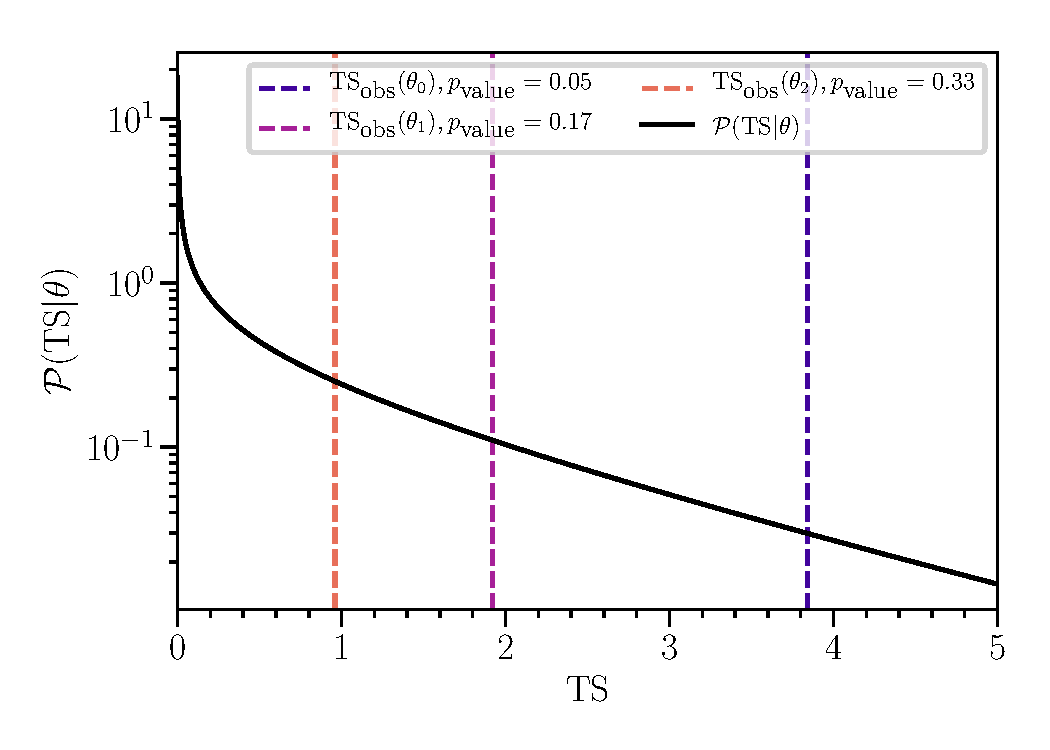
\includegraphics[width=0.8\linewidth]{figures/TS_dist}
	\caption{\textbf{\textit{Test statistic distribution.}} An example of a test statistic distribution.
	Such distributions tend to have the bulk of their mass close to the lower boundary with a long tail.
	Lower values indicate better statistical compatibility with the data.
	}
	\label{fig:TS_dist}
\end{figure}
It is important to note that for the profile likelihood TS and similar statistics a smaller TS value indicates better compatibility with the data.
For this reason many statistical tests are constructed using a single tail significance, by comparing the TS from a single experiment to a background TS distribution and reporting a p-value that is the fraction of the TS distribution greater than the observed TS.

This procedure can be extended to construct intervals by considering the TS distributions of every point in parameter space and comparing to the observed TS function.
Consider the one-dimensional case where there is a TS distribution for each value of the parameter, illustrated in~\reffig{fig:TS_dists_1d}
\begin{figure}
	\centering
	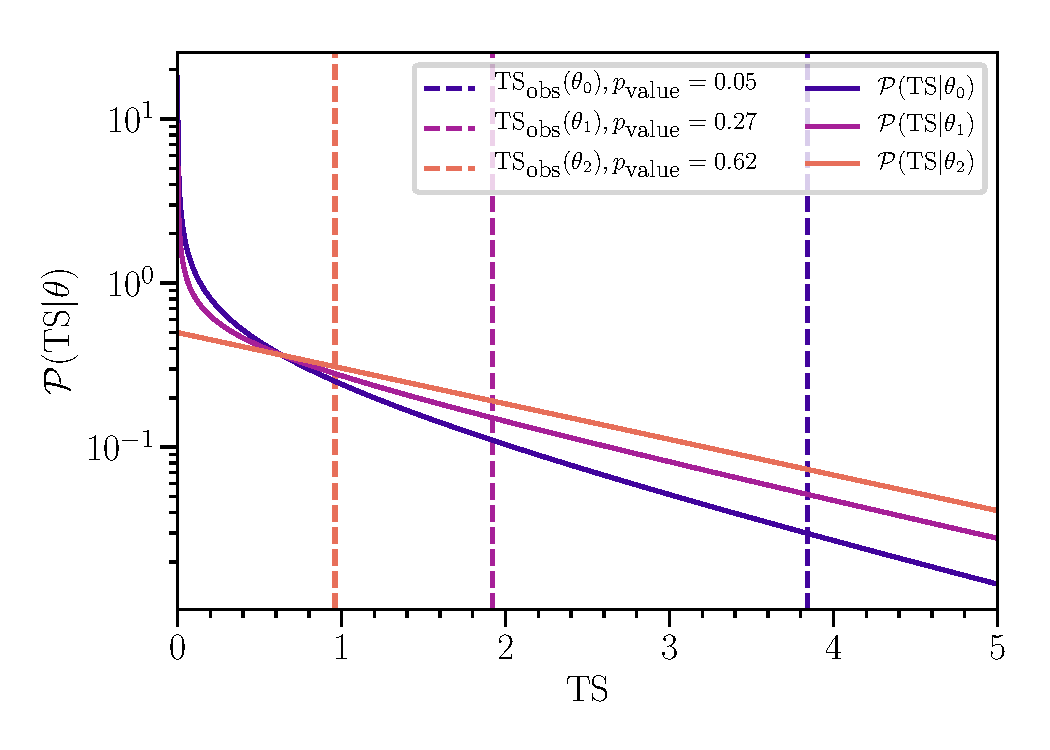
\includegraphics[width=0.8\linewidth]{figures/TS_dists_1d}
	\caption{\textbf{\textit{One-dimensional test-statistic distribution comparison.}} An example of the test statistic distributions as a function of a single parameter.
	}
	\label{fig:TS_dists_1d}
\end{figure}
We can construct an interval that will contain the true value of the parameter a fraction of the time $\alpha$ for repeated experiments.
This interval is the collection of points in the one-dimensional parameter space where the TS at that point is greater than the $\alpha$ quantile of the corresponding TS distribution.
If the TS distribution is the same for all points in parameter space, the interval construction can procedurally be thought of as drawing a horizontal line at the appropriate threshold and only including points that lie below the line.
Varying TS distributions modify this procedure to the comparison of two curves.
This procedure is not limited to one-dimension but can be extended to an arbitrary number of parameters of interest to construct n-dimensional regions with the same properties.

There is however an important caveat to this construction that appears when we consider nuisance parameters.
In order for the intervals to have the desired properties, the observed TS must be greater than the threshold for all possible values of the nuisance parameters.
This ultimatum presents several challenges.
Nuisance parameters can often have a broad or even unbounded range of allowed values, meaning if the effect of nuisance parameters does not taper off at the extrema then almost all intervals are guaranteed to be empty.
From a practical standpoint, computing the TS distributions for many points in parameter space is often done via Monte-Carlo and is computationally expensive.
Adding additional dimensions to the parameter space for which we must compute TS distributions exponentially increases the computation time.

To combat these issues we can limit our interval construction to be valid for values of the nuisance parameters that are ``reasonable''.
There are several methods for doing this, but we can split them into two categories: pure frequentist, and frequentist-Bayesian hybrid.
In the pure frequentist approaches we can either choose a single value of the nuisance parameters, or work with a limited range of the nuisance parameter values.
For the single value approach either nominal values are chosen before looking at the data, or estimators of the nuisance parameters are used to choose their values.
This approach benefits from simplicity, but fails if the test-statistic distributions vary rapidly with changes to the nuisance parameters for values that we might consider ``reasonable''.
A more expensive but robust approach is to explore the behavior of TS distributions for a limited range of the nuisance parameter values, which can be chosen {\it a priori} or from data-based bounds on the nuisance parameters.
If we are willing to consider a hybrid approach, then some more pragmatic options are available.

Although Bayesian methods could be used to choose a single point in parameter space from which to generate the TS distributions, the more interesting application is one that uses a distribution in parameter space.
In Bayesian statistics we can directly assign a probability density to the points in parameter space, either based on our prior information, or directly informed by the posterior distribution, from this extended perspective the probability of certain nuisance parameter values is of interest when considering the frequency of TS values for different parameters of interest.
The prior case is simple in that we sample the from the nuisance parameter priors when generating the TS distribution which allows us to account for variability introduced by the nuisance parameters without relying on hard cutoffs or biasing our inferences with parameter values that are unrealistic.
This prior based technique is well motivated if the priors are derived from external observations, however in the case where nuisance parameters have broad or ``uninformative'' priors this motivation and benefit may break down.
In some cases we expect nuisance parameters to be heavily constrained by the same data sample used to investigate the parameters of interest, so a different approach is merited.
The alternative is to use the posterior distribution to construct our nuisance parameter p.d.f.
Ideally a posterior distribution would be computed for each point in the parameters of interest space by fixing those parameters of interest.
In this way the nuisance parameter posterior used for sampling depends on the point in parameter space we are examining.

With the possible solutions available, we can now look at the problem of limited simulation size when generating test statistic distributions.
As explored in~\refsec{sec:limited_simulation} for binned Poisson likelihood problems, the real expectation in data or simulation for the number of events in a bin is not a known quantity.
Because the real expectations are not known, it is impossible to exactly model the distribution of TS that are expected for a particular point in the parameter space.
However, as~\refsec{sec:limited_simulation} also explored, limited simulation can be modeled with nuisance parameters so the techniques discussed above can be applied directly to the problem.
The ``single point in parameter space'' approach fails to address the additional uncertainty present in this case.
Allowing for unbounded variation of the bin expectations fails as it is guaranteed to produce empty intervals.
Bounding of the bin expectations within a reasonable range provides manageable intervals, but the dimensionality of the problem makes this computationally unfeasible beyond a handful of bins.
Unfortunately this excludes all the ``classic'' frequentist solutions to this problem.
The hybrid Bayesian-frequentist methods in this case provide a tractable solution that accounts for the additional uncertainty.
We can make use of the treatment described in~\refsec{sec:effective}, where the bin expectation is derived to be gamma distributed, and the expected number of data events modeled to be Poisson distributed once this expectation is known.
Practically this can be achieved by sampling data events from $\mcl$, or through a two step process where the expectation is sampled from a gamma distribution $\gprob(\lambda;\agpar, \bgpar)$ where $\agpar = \frac{\mu^2}{\sigma^2}+1~\textmd{and}~\bgpar=\frac{\mu}{\sigma^2}$, and the data events are sampled from a Poisson distribution $\frac{\lambda^{k}e^{-\lambda}}{k!}$.
It is important to note that this procedure only applies to variations in the data and should not be used to vary simulation expectations.
This is because the TS distribution is intended to model variations in the data, whereas the simulation used for analysis is fixed.
Combined with a similar hybrid treatment for other nuisance parameters, this provides a more complete accounting of the uncertainties given the available modeling.
\endgroup

\section{Dealing with limited simulation samples\label{sec:limited_simulation}}
The contents of this section is reproduced here with minor modifications from a collaborative work with Carlos A. Argüelles, and Tianlu Yuan~\cite{Arguelles:2019izp}.

\begingroup
\graphicspath{{results/mcllh_paper/}}
\chapter{Introduction}


\endgroup

\subsection{The Poisson likelihood and previous work\label{sec:mc_intro}}
\begingroup
\graphicspath{{results/mcllh_paper/}}
\input{results/mcllh_paper/sections/previous_work/poisson}
\endgroup

\subsubsection{The Barlow-Beeston likelihood}
\begingroup
\graphicspath{{results/mcllh_paper/}}
\input{results/mcllh_paper/sections/previous_work/bb}
\endgroup

\subsubsection{Uncertainties in the large-sample limit}
\begingroup
\graphicspath{{results/mcllh_paper/}}
\input{results/mcllh_paper/sections/previous_work/chi2}
\endgroup

\subsection{Generalization of the Poisson likelihood\label{sec:generalization_poisson}}
\begingroup
\graphicspath{{results/mcllh_paper/}}
\input{results/mcllh_paper/sections/generalized_poisson/generalized_poisson}
\endgroup

\subsubsection{Derivation of $\like (\lambda|\vecw(\vectheta))$ for identical weights\label{sec:constructing}}
\begingroup
\graphicspath{{results/mcllh_paper/}}
\input{results/mcllh_paper/sections/generalized_poisson/identical_weights}
\endgroup

\subsubsection{Extension to arbitrary weights\label{sec:extending}}
\begingroup
\graphicspath{{results/mcllh_paper/}}
\input{results/mcllh_paper/sections/generalized_poisson/arbitrary_weights}
\endgroup

\subsubsection{The effective likelihood\label{sec:effective}}
\begingroup
\graphicspath{{results/mcllh_paper/}}
\input{results/mcllh_paper/sections/generalized_poisson/effective_likelihood}
\endgroup

\subsubsection{A family of likelihoods\label{sec:priors}}
\begingroup
\graphicspath{{results/mcllh_paper/}}
\input{results/mcllh_paper/sections/generalized_poisson/family}
\endgroup

\subsubsection{Convergence of the effective likelihood\label{sec:llhconvergence}}
\begingroup
\graphicspath{{results/mcllh_paper/}}
\input{results/mcllh_paper/sections/generalized_poisson/convergence}
\endgroup

\subsubsection{Behavior of the effective likelihood\label{sec:llhbehavior}}
\begingroup
\graphicspath{{results/mcllh_paper/}}
\input{results/mcllh_paper/sections/generalized_poisson/behavior}
\endgroup

\subsection{Example and performance\label{sec:example}}
\begingroup
\graphicspath{{results/mcllh_paper/}}
\input{results/mcllh_paper/sections/example/example}
\endgroup

\subsubsection{Point estimation\label{sec:pointestimation}}
\begingroup
\graphicspath{{results/mcllh_paper/}}
\input{results/mcllh_paper/sections/example/point_estimation}
\endgroup

\subsubsection{Coverage\label{sec:coverage}}
\begingroup
\graphicspath{{results/mcllh_paper/}}
\input{results/mcllh_paper/sections/example/coverage}
\endgroup

\subsubsection{Posterior distributions\label{sec:posterior}}
\begingroup
\graphicspath{{results/mcllh_paper/}}
\input{results/mcllh_paper/sections/example/posterior}
\endgroup

\subsubsection{Performance\label{sec:performance}}
\begingroup
\graphicspath{{results/mcllh_paper/}}
\input{results/mcllh_paper/sections/example/performance}
\endgroup

\subsection{Conclusion\label{sec:llhconclusion}}
\begingroup
\graphicspath{{results/mcllh_paper/}}
\input{results/mcllh_paper/sections/conclusion}
\endgroup

\subsection{Summary of likelihood formulas\label{sec:llhtable}}
\begingroup
\graphicspath{{results/mcllh_paper/}}
\input{results/mcllh_paper/appendices/formulas}
\endgroup
\FloatBarrier
\section{Frequentist confidence intervals with nuisance parameters and limited simulation}\label{sec:low_stats_confidence_intervals}

Frequentist and Bayesian techniques deal with different two different kinds of probability.
In frequentist statistics, the relevant probability is the frequency of the outcome of a repeatable experiment.
Under this framework the important concepts are parameter estimation, confidence intervals, and statistical tests.
In Bayesian statistics, the relevant probabilities come from the application of Bayes theorem which means we can define the probability density of parameters.
This definition of the parameter p.d.f. is applicable to the same problems parameter estimation, interval construction, and statistical tests but comes at the cost of defining ``prior belief'' about parameters.

In this section we will ignore the problem of statistical tests, instead focusing on the common features that underpin parameter estimation and interval construction.
Generally in parameter estimation and interval construction there are two sets of parameters, parameters of interest $\vec\theta$ and nuisance parameters $\vec\eta$.
Fundamentally there is no distinction between these two kinds of parameters.
The difference is only in which parameters we want to infer information about.

For both parameter estimation and interval construction the likelihood function is central.
The likelihood function reflects the plausibility of model parameters given observed data and is defined as $\like(\vec\theta, \vec\eta|\textrm{data}) = p(\textrm{data}|\vec\theta, \vec\eta)$.
Where $p(\textrm{data}|\vec\theta, \vec\eta)$ is the probability of the data given the model parameters.
A useful technique to eliminate nuisance parameters is the profile likelihood technique.
Dropping the explicit notational dependence on data, the profile likelihood function is defined as
\begin{linenomath*}
	\begin{equation}
	\tilde{\like}^\texttt{profile}(\vec\theta) = \max_{\vec\eta} \like(\vec\theta,\vec\eta),
	\label{eq:likelihood_profile}
	\end{equation}
\end{linenomath*}
where often the negative log of the function is maximized in place of the function for computational reasons.
The profile likelihood is then only a function of the parameters of interest.
Parameter estimation can be performed by maximizing the profile likelihood to obtain the ``best-fit'' parameters
\begin{linenomath*}
	\begin{equation}
	\hat{\vec\theta} = \argmax_{\vec\theta} \tilde{\like}^\texttt{profile}(\vec\theta).
	\label{eq:best_fit}
	\end{equation}
\end{linenomath*}
This best-fit point in the parameter space is a derived property of the likelihood function.
However, the same procedure can be performed with other functions to the same effect.
In general a minimization procedure is used, and we refer to these functions as ``test-statistics'' (TS).
A particularly useful TS is derived directly from the profile likelihood technique,
\begin{linenomath*}
	\begin{equation}
	\TS(\vec\theta) = -2\log{\left(\frac{\tilde{\like}^\texttt{profile}(\vec\theta)}{\tilde{\like}^\texttt{profile}(\hat{\vec\theta})}\right)}.
	\end{equation}
\end{linenomath*}
Using this TS to perform parameter estimation through minimization is mathematically equivalent to maximizing the likelihood, however, this form will prove to be uniquely useful for interval construction.

Since frequentist statistics deals with the frequency of outcomes from repeated experiments we can use the TS that results from repeated experiments to construct probabilities.
Consider for a moment a single point in the parameter space $\vec\theta_0$.
At this point in the parameter space there is a distribution of data that can be observed, and therefore a distribution of TS functions.
Instead of considering the distribution of TS functions originating from this point, we can simplify the picture by looking at the TS function only evaluated at this point $\TS(\vec\theta_0)$.
This gives us a distribution of TS values for this point in the parameter space that may look like~\reffig{fig:TS_dist}.
\begin{figure}
	\centering
	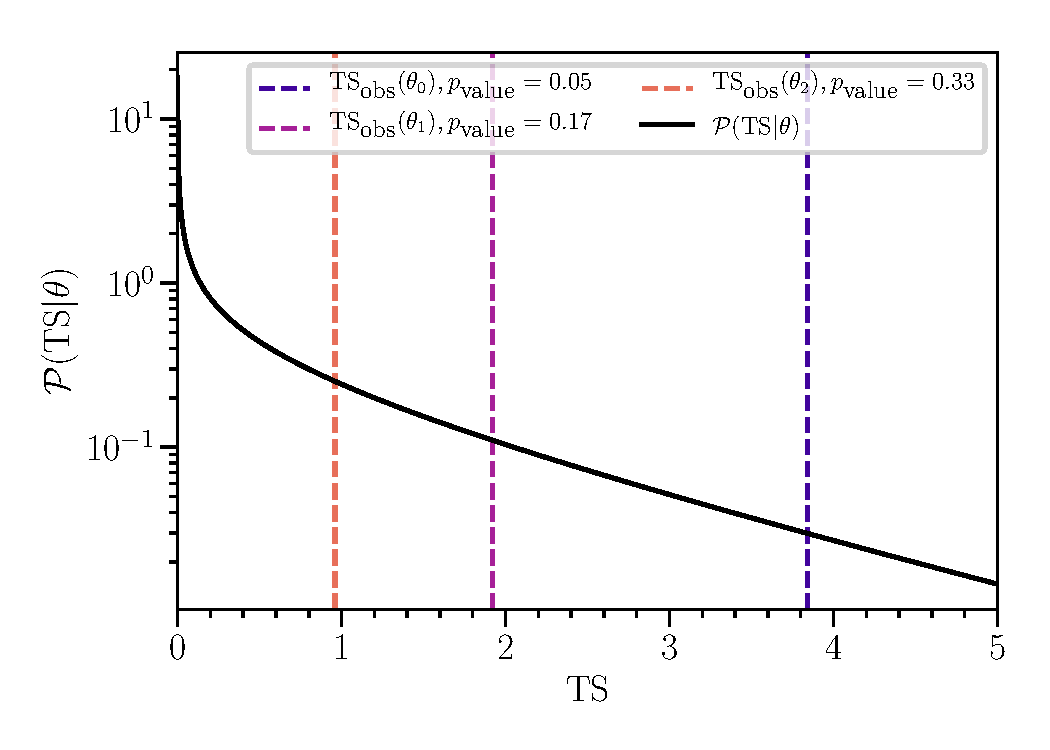
\includegraphics[width=0.8\linewidth]{figures/TS_dist}
	\caption{\textbf{\textit{Test statistic distribution.}} An example of a test statistic distribution.
	Such distributions tend to have the bulk of their mass close to the lower boundary with a long tail.
	Lower values indicate better statistical compatibility with the data.
	}
	\label{fig:TS_dist}
\end{figure}
It is important to note that for the profile likelihood TS and similar statistics a smaller TS value indicates better compatibility with the data.
For this reason many statistical tests are constructed using a single tail significance, by comparing the TS from a single experiment to a background TS distribution and reporting a p-value that is the fraction of the TS distribution greater than the observed TS.

This procedure can be extended to construct intervals by considering the TS distributions of every point in parameter space and comparing to the observed TS function.
Consider the one-dimensional case where there is a TS distribution for each value of the parameter, illustrated in~\reffig{fig:TS_dists_1d}
\begin{figure}
	\centering
	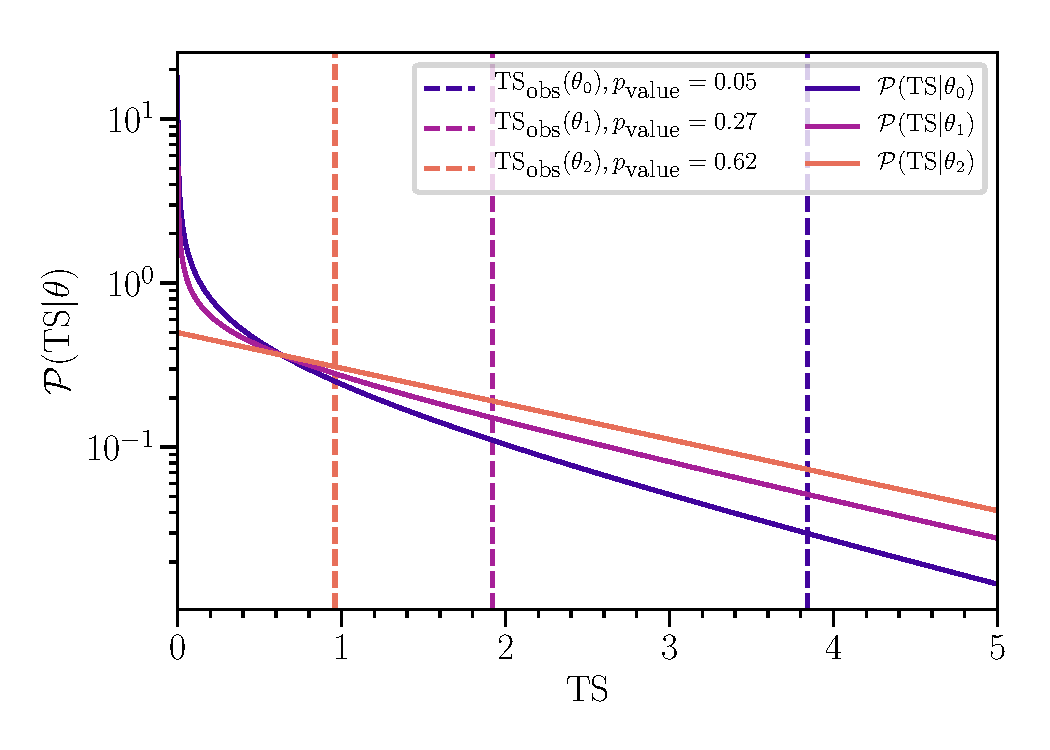
\includegraphics[width=0.8\linewidth]{figures/TS_dists_1d}
	\caption{\textbf{\textit{One-dimensional test-statistic distribution comparison.}} An example of the test statistic distributions as a function of a single parameter.
	}
	\label{fig:TS_dists_1d}
\end{figure}
We can construct an interval that will contain the true value of the parameter a fraction of the time $\alpha$ for repeated experiments.
This interval is the collection of points in the one-dimensional parameter space where the TS at that point is greater than the $\alpha$ quantile of the corresponding TS distribution.
If the TS distribution is the same for all points in parameter space, the interval construction can procedurally be thought of as drawing a horizontal line at the appropriate threshold and only including points that lie below the line.
Varying TS distributions modify this procedure to the comparison of two curves.
This procedure is not limited to one-dimension but can be extended to an arbitrary number of parameters of interest to construct n-dimensional regions with the same properties.

There is however an important caveat to this construction that appears when we consider nuisance parameters.
In order for the intervals to have the desired properties, the observed TS must be greater than the threshold for all possible values of the nuisance parameters.
This ultimatum presents several challenges.
Nuisance parameters can often have a broad or even unbounded range of allowed values, meaning if the effect of nuisance parameters does not taper off at the extrema then almost all intervals are guaranteed to be empty.
From a practical standpoint, computing the TS distributions for many points in parameter space is often done via Monte-Carlo and is computationally expensive.
Adding additional dimensions to the parameter space for which we must compute TS distributions exponentially increases the computation time.

To combat these issues we can limit our interval construction to be valid for values of the nuisance parameters that are ``reasonable''.
There are several methods for doing this, but we can split them into two categories: pure frequentist, and frequentist-Bayesian hybrid.
In the pure frequentist approaches we can either choose a single value of the nuisance parameters, or work with a limited range of the nuisance parameter values.
For the single value approach either nominal values are chosen before looking at the data, or estimators of the nuisance parameters are used to choose their values.
This approach benefits from simplicity, but fails if the test-statistic distributions vary rapidly with changes to the nuisance parameters for values that we might consider ``reasonable''.
A more expensive but robust approach is to explore the behavior of TS distributions for a limited range of the nuisance parameter values, which can be chosen {\it a priori} or from data-based bounds on the nuisance parameters.
If we are willing to consider a hybrid approach, then some more pragmatic options are available.

Although Bayesian methods could be used to choose a single point in parameter space from which to generate the TS distributions, the more interesting application is one that uses a distribution in parameter space.
In Bayesian statistics we can directly assign a probability density to the points in parameter space, either based on our prior information, or directly informed by the posterior distribution, from this extended perspective the probability of certain nuisance parameter values is of interest when considering the frequency of TS values for different parameters of interest.
The prior case is simple in that we sample the from the nuisance parameter priors when generating the TS distribution which allows us to account for variability introduced by the nuisance parameters without relying on hard cutoffs or biasing our inferences with parameter values that are unrealistic.
This prior based technique is well motivated if the priors are derived from external observations, however in the case where nuisance parameters have broad or ``uninformative'' priors this motivation and benefit may break down.
In some cases we expect nuisance parameters to be heavily constrained by the same data sample used to investigate the parameters of interest, so a different approach is merited.
The alternative is to use the posterior distribution to construct our nuisance parameter p.d.f.
Ideally a posterior distribution would be computed for each point in the parameters of interest space by fixing those parameters of interest.
In this way the nuisance parameter posterior used for sampling depends on the point in parameter space we are examining.

With the possible solutions available, we can now look at the problem of limited simulation size when generating test statistic distributions.
As explored in~\refsec{sec:limited_simulation} for binned Poisson likelihood problems, the real expectation in data or simulation for the number of events in a bin is not a known quantity.
Because the real expectations are not known, it is impossible to exactly model the distribution of TS that are expected for a particular point in the parameter space.
However, as~\refsec{sec:limited_simulation} also explored, limited simulation can be modeled with nuisance parameters so the techniques discussed above can be applied directly to the problem.
The ``single point in parameter space'' approach fails to address the additional uncertainty present in this case.
Allowing for unbounded variation of the bin expectations fails as it is guaranteed to produce empty intervals.
Bounding of the bin expectations within a reasonable range provides manageable intervals, but the dimensionality of the problem makes this computationally unfeasible beyond a handful of bins.
Unfortunately this excludes all the ``classic'' frequentist solutions to this problem.
The hybrid Bayesian-frequentist methods in this case provide a tractable solution that accounts for the additional uncertainty.
We can make use of the treatment described in~\refsec{sec:effective}, where the bin expectation is derived to be gamma distributed, and the expected number of data events modeled to be Poisson distributed once this expectation is known.
Practically this can be achieved by sampling data events from $\mcl$, or through a two step process where the expectation is sampled from a gamma distribution $\gprob(\lambda;\agpar, \bgpar)$ where $\agpar = \frac{\mu^2}{\sigma^2}+1~\textmd{and}~\bgpar=\frac{\mu}{\sigma^2}$, and the data events are sampled from a Poisson distribution $\frac{\lambda^{k}e^{-\lambda}}{k!}$.
It is important to note that this procedure only applies to variations in the data and should not be used to vary simulation expectations.
This is because the TS distribution is intended to model variations in the data, whereas the simulation used for analysis is fixed.
Combined with a similar hybrid treatment for other nuisance parameters, this provides a more complete accounting of the uncertainties given the available modeling.